The second model examined was introduced by Chen et al. \cite{chen2021shape}, 
building on the prior work of Spagnolie et al. 
\cite{spagnolie2015geometric}. This model extends the previous analysis by explicitly incorporating hydrodynamic
interactions between the channel walls into the governing SDEs.

Spagnolie et al. approximate the velocity field surrounding an elliptical microswimmer by treating it 
first as a \textit{stresslet} - a force dipole - and then applying Faxén's Law to derive the 
correpsonding velocity field associated with an elliptical stresslet. Figures \ref{fig:model_2_intro} 
illustrates the microswimmer as a stresslet and the velocity field generated by such an elliptical swimmer,
near a circular boundary.


\begin{figure}[htbp]
    \centering
    \begin{subfigure}[b]{0.45\textwidth}
        \centering
        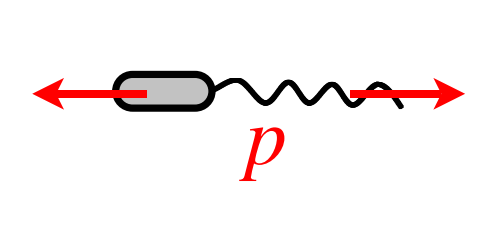
\includegraphics[width=\textwidth]{graphics/pusher_pic.png}
        \caption{Representation of a \textit{pusher} microswimmer as a stresslet \(force dipole\).}
        \label{fig:pusher_chart}
    \end{subfigure}
    \hfill
    \begin{subfigure}[b]{0.45\textwidth}
        \centering
        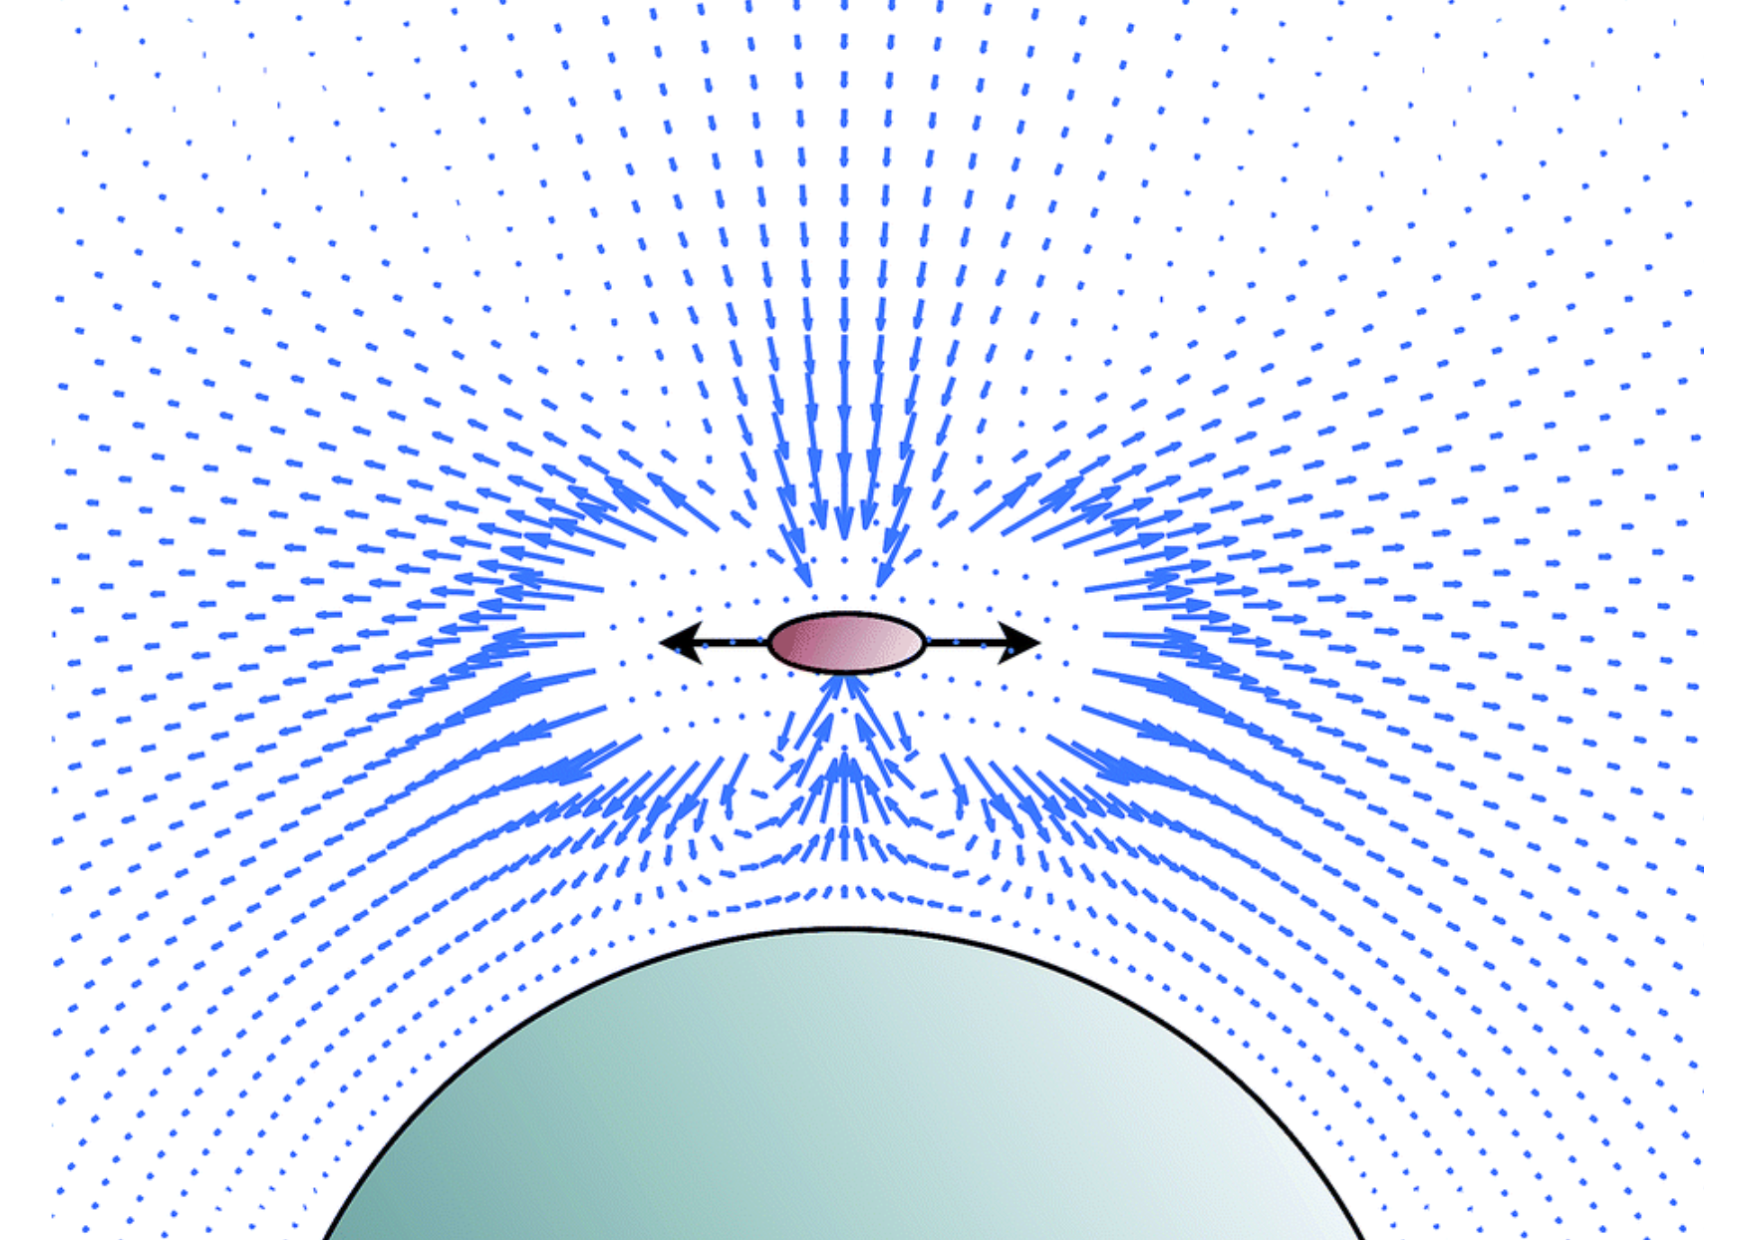
\includegraphics[width=\textwidth]{graphics/fluid_field_model2.pdf}
        \caption{Fluid velocity field around a pusher microswimmer near a boundary. Image
        adapted from \cite{spagnolie2015geometric}}
        \label{fig:fluid_field_pusher}
    \end{subfigure}
    \caption{Visual depiction of key components in hydrodynamic model.}
    \label{fig:model_2_intro}
\end{figure}

Microswimmers are commonly classified as either 
\textit{pushers} or \textit{pullers}, based on whether they propel themselves by pushing fluid 
back or pulling fluid forward \cite{berke2008hydrodynamic}. In this analysis we consider solely pusher-type microswimmers.

Spagnolie et al. derived hydrodynamic equations describing the boundary-induced effects on the cell's motion
near a circular boundary:

\begin{subequations}
    \begin{align}\label{eq:hydrodynamic_circular_eqs}
        \frac{dr}{dt} &= \sin(\theta) - \frac{3\alpha}{8r^2}(1-3\sin^2(\theta)) \\
        \frac{d\theta}{dt} &= \frac{1}{A}-\frac{3\alpha}{64r^3}[4 - \Gamma(3-cos(2\theta))]\sin(2\theta)
    \end{align}        
\end{subequations}

where $\alpha$ denotes the dipole strength, with $\alpha > 0$ for pushers and $\alpha < 0$ for pullers 
\cite{berke2008hydrodynamic}, $\Gamma$ is the aspect ratio of the elliptical microswimmer, 
$A$ is the radius of the circular boundary and $r$ is the distance from this boundary.

For the scenario considered in this report - an elliptical swimmer within an infinite channel 
bounded above and below by parallel walls - we take the limit as $A \to \infty$.
In this limit, we define the vertical distance $y$ from the cell centre to the channel walls 
along the $y$-axis. The resulting modified equations are given by Chen et al. \cite{chen2021shape} as:

\begin{subequations}\label{eq:modified_hydrodynamic_eqs}
    \begin{align}
        \frac{dy}{dt} &= \sin(\theta) - \frac{3\alpha}{8h^2}
        \big(\frac{a^2}{y^2}-\frac{a^2}{(H - y)^2}\big)(1-3\sin^2(\theta)) \\
        \frac{d\theta}{dt} &= -\frac{3\alpha}{64y^3}\big(\frac{a^3}{y^3} + \frac{a^3}{(H-y)^3}\big)
        [4 - \Gamma(3-\cos(2\theta))]\sin(2\theta).
    \end{align}    
\end{subequations}

 Where $H$ is the fixed channel height. 
 
 Incorporating equations \eqref{eq:modified_hydrodynamic_eqs} into the stochastic framework
 established in model 1 \eqref{eq:model1_sdes}, we obtain the following system of SDEs describing 
 the swimmers dynamics:

\begin{subequations}\label{eq:model_2_sdes}
    \begin{align}
        Y(t + \Delta t) &= Y(t) + U \sin(\theta)\Delta t - \frac{3U\alpha}{8}\big(\frac{a^2}{y^2}-\frac{a^2}{(H-y)^2}\big)
        (1-3\sin^2(\theta))\Delta t + \sqrt{2D_y}\Delta W_1 \\
        \theta(t + \Delta t) &= \theta(t) -\frac{3U\alpha}{64\alpha} \big(\frac{a^3}{y^3} + 
        \frac{a^3}{(H-y)^3}\big)[4-\Gamma(3-\cos(2\theta))]
        \sin(2\theta) \Delta t + \sqrt{2D_{\theta}}\Delta W_2
     \end{align}
\end{subequations}

Monte-Carlo simulations were performed to obtain the stationary marginal
distributions associated with \eqref{eq:model_2_sdes}. 
These distributions are presented in Figure \ref{fig:model_2_results}.

\begin{figure}[htbp]
    \centering
    \begin{subfigure}[b]{0.45\textwidth}
        \centering
        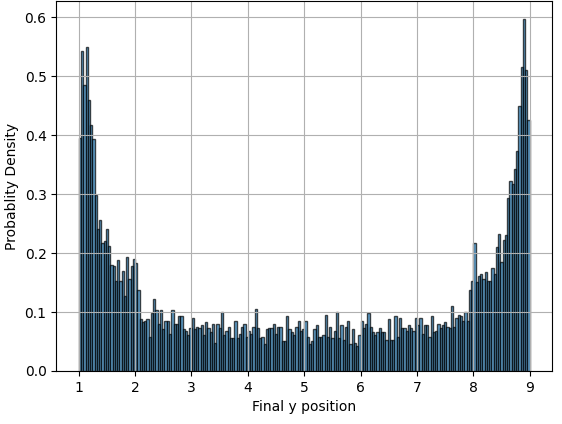
\includegraphics[width=\textwidth]{graphics/model_2_y_dist.png}
        \caption{Distribution across $y$.}
        \label{fig:model_2_y_hist}
    \end{subfigure}
    \hfill
    \begin{subfigure}[b]{0.45\textwidth}
        \centering
        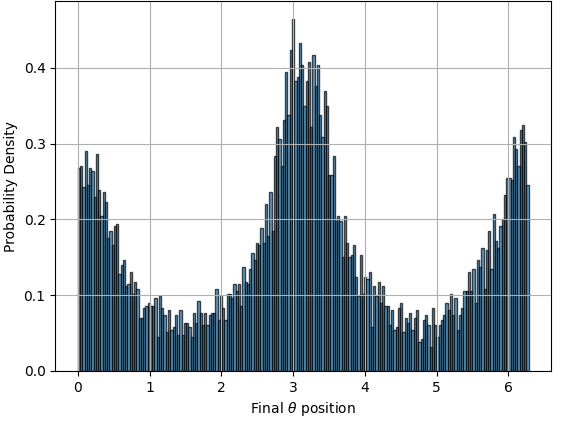
\includegraphics[width=\textwidth]{graphics/model_2_theta_dist.png}
        \caption{Distribution across $\theta$.}
        \label{fig:model_2_theta_hist}
    \end{subfigure}
    \caption{Marginal distributions obtained via 
    Monte Carlo simulation from equations \eqref{eq:model_2_sdes}}
    \label{fig:model_2_results}
\end{figure}

It can be observed that the same characteristic accummulation at the boundaries is obtained in the
$y$ distribution. Additionally, the angular distribution
exhibits notable peaks at $0$, $\pi$, and $2\pi$. This corresponds to cases where the cell is 
aligned parallel to the channel walls, highlighting a preferred orientation arising from hydrodynamic
interactions.







